\subsection{Unlocking the Secrets of Receiver's Blocking Dynamic Range!}

\begin{tcolorbox}[colback=gray!10, colframe=black, title=E4D01] What is meant by the blocking dynamic range of a receiver?
\begin{enumerate}[label=\Alph*.]
    \item \textbf{The difference in dB between the noise floor and the level of an incoming signal that will cause 1 dB of gain compression}
    \item The minimum difference in dB between the levels of two FM signals that will cause one signal to block the other
    \item The difference in dB between the noise floor and the third-order intercept point
    \item The minimum difference in dB between two signals which produce third-order intermodulation products greater than the noise floor
\end{enumerate} \end{tcolorbox}

\subsubsection{Concepts Related to the Blocking Dynamic Range}

The blocking dynamic range is a crucial parameter in radio communications, specifically in the performance of receivers. It measures how effectively a receiver can operate amidst signals that may interfere with its ability to discern the desired signal from unwanted noise or other signals.

To understand this concept fully, let's break it down:

1. \textbf{Noise Floor}: This is the level of background noise present at the receiver. It is typically measured in decibels (dB) and represents the minimum signal level that can be detected.

2. \textbf{Gain Compression}: When a signal level reaches a certain point, the receiver's amplification begins to compress the gain. A common metric used is a 1 dB compression point, which indicates at what level the gain is reduced by 1 dB compared to its linear response.

3. \textbf{Blocking}: In the context of multiple signals being received, blocking refers to the scenario where one strong signal interferes with the receiver's ability to process a weaker, desired signal. 

4. \textbf{Intermodulation}: This occurs when two or more signals mix within a nonlinear system, producing signals at new frequencies, which may fall within or near the frequency range of the desired signal.

The correct answer provided, option A, states that the blocking dynamic range is:

\textbf{The difference in dB between the noise floor and the level of an incoming signal that will cause 1 dB of gain compression.}

This definition implies that a receiver's ability to differentiate between signals is limited by both the noise it must work against (noise floor) and the level of incoming signals that can lead to distortion (gain compression).

\subsubsection{Calculation Example}

Let's assume a receiver has the following specifications:
- Noise floor: -100 dBm
- 1 dB compression point occurs at -50 dBm

To find the blocking dynamic range, we can calculate it as follows:

\[
\text{Blocking Dynamic Range} = \text{Compression Point} - \text{Noise Floor}
\]

Substituting the values:

\[
\text{Blocking Dynamic Range} = (-50 \, \text{dBm}) - (-100 \, \text{dBm}) = -50 \, \text{dBm} + 100 \, \text{dBm} = 50 \, \text{dB}
\]

Thus, the blocking dynamic range of this particular receiver would be 50 dB.

\subsubsection{Diagram}

To visualize these concepts, we can draw a simple diagram using TikZ:

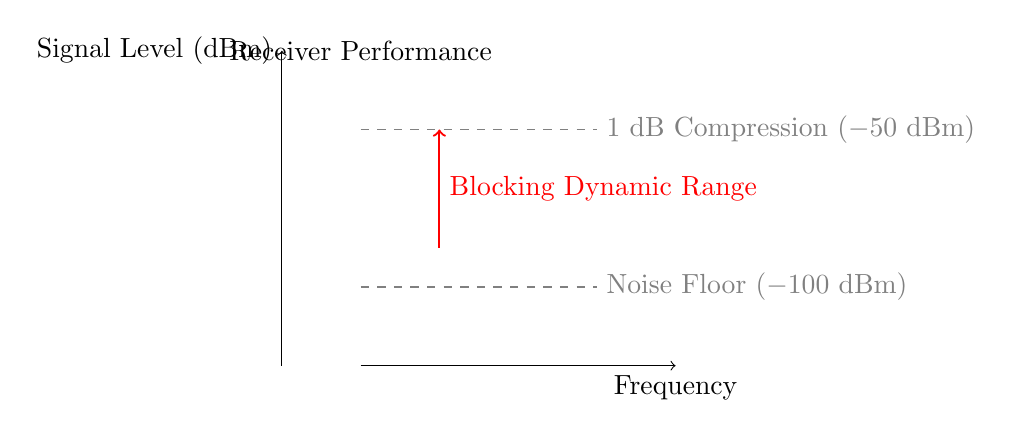
\begin{tikzpicture}
    % Axis
    \draw[->] (-1,0) -- (-1,4) node[left] {Signal Level (dBm)};
    \draw[->] (0,0) -- (4,0) node[below] {Frequency};

    % Noise floor
    \draw[dashed, gray] (0,1) -- (3,1) node[right] {Noise Floor ($-100$ dBm)};
    
    % Compression point
    \draw[dashed, gray] (0,3) -- (3,3) node[right] {1 dB Compression ($-50$ dBm)};
    
    % Indicator for blocking range
    \draw[thick, red, ->] (1,1.5) -- (1,3) node[midway,right] {Blocking Dynamic Range};

    % Labels
    \node at (0, 4) {Receiver Performance};
\end{tikzpicture}
